\documentclass[]{article}
\usepackage{lmodern}
\usepackage{amssymb,amsmath}
\usepackage{ifxetex,ifluatex}
\usepackage{fixltx2e} % provides \textsubscript
\ifnum 0\ifxetex 1\fi\ifluatex 1\fi=0 % if pdftex
  \usepackage[T1]{fontenc}
  \usepackage[utf8]{inputenc}
\else % if luatex or xelatex
  \ifxetex
    \usepackage{mathspec}
  \else
    \usepackage{fontspec}
  \fi
  \defaultfontfeatures{Ligatures=TeX,Scale=MatchLowercase}
\fi
% use upquote if available, for straight quotes in verbatim environments
\IfFileExists{upquote.sty}{\usepackage{upquote}}{}
% use microtype if available
\IfFileExists{microtype.sty}{%
\usepackage{microtype}
\UseMicrotypeSet[protrusion]{basicmath} % disable protrusion for tt fonts
}{}
\usepackage[margin=1in]{geometry}
\usepackage{hyperref}
\hypersetup{unicode=true,
            pdftitle={Predicting Household Composition by TV Viewing Behavior},
            pdfauthor={Rafael Lüchinger},
            pdfborder={0 0 0},
            breaklinks=true}
\urlstyle{same}  % don't use monospace font for urls
\usepackage{color}
\usepackage{fancyvrb}
\newcommand{\VerbBar}{|}
\newcommand{\VERB}{\Verb[commandchars=\\\{\}]}
\DefineVerbatimEnvironment{Highlighting}{Verbatim}{commandchars=\\\{\}}
% Add ',fontsize=\small' for more characters per line
\usepackage{framed}
\definecolor{shadecolor}{RGB}{248,248,248}
\newenvironment{Shaded}{\begin{snugshade}}{\end{snugshade}}
\newcommand{\KeywordTok}[1]{\textcolor[rgb]{0.13,0.29,0.53}{\textbf{#1}}}
\newcommand{\DataTypeTok}[1]{\textcolor[rgb]{0.13,0.29,0.53}{#1}}
\newcommand{\DecValTok}[1]{\textcolor[rgb]{0.00,0.00,0.81}{#1}}
\newcommand{\BaseNTok}[1]{\textcolor[rgb]{0.00,0.00,0.81}{#1}}
\newcommand{\FloatTok}[1]{\textcolor[rgb]{0.00,0.00,0.81}{#1}}
\newcommand{\ConstantTok}[1]{\textcolor[rgb]{0.00,0.00,0.00}{#1}}
\newcommand{\CharTok}[1]{\textcolor[rgb]{0.31,0.60,0.02}{#1}}
\newcommand{\SpecialCharTok}[1]{\textcolor[rgb]{0.00,0.00,0.00}{#1}}
\newcommand{\StringTok}[1]{\textcolor[rgb]{0.31,0.60,0.02}{#1}}
\newcommand{\VerbatimStringTok}[1]{\textcolor[rgb]{0.31,0.60,0.02}{#1}}
\newcommand{\SpecialStringTok}[1]{\textcolor[rgb]{0.31,0.60,0.02}{#1}}
\newcommand{\ImportTok}[1]{#1}
\newcommand{\CommentTok}[1]{\textcolor[rgb]{0.56,0.35,0.01}{\textit{#1}}}
\newcommand{\DocumentationTok}[1]{\textcolor[rgb]{0.56,0.35,0.01}{\textbf{\textit{#1}}}}
\newcommand{\AnnotationTok}[1]{\textcolor[rgb]{0.56,0.35,0.01}{\textbf{\textit{#1}}}}
\newcommand{\CommentVarTok}[1]{\textcolor[rgb]{0.56,0.35,0.01}{\textbf{\textit{#1}}}}
\newcommand{\OtherTok}[1]{\textcolor[rgb]{0.56,0.35,0.01}{#1}}
\newcommand{\FunctionTok}[1]{\textcolor[rgb]{0.00,0.00,0.00}{#1}}
\newcommand{\VariableTok}[1]{\textcolor[rgb]{0.00,0.00,0.00}{#1}}
\newcommand{\ControlFlowTok}[1]{\textcolor[rgb]{0.13,0.29,0.53}{\textbf{#1}}}
\newcommand{\OperatorTok}[1]{\textcolor[rgb]{0.81,0.36,0.00}{\textbf{#1}}}
\newcommand{\BuiltInTok}[1]{#1}
\newcommand{\ExtensionTok}[1]{#1}
\newcommand{\PreprocessorTok}[1]{\textcolor[rgb]{0.56,0.35,0.01}{\textit{#1}}}
\newcommand{\AttributeTok}[1]{\textcolor[rgb]{0.77,0.63,0.00}{#1}}
\newcommand{\RegionMarkerTok}[1]{#1}
\newcommand{\InformationTok}[1]{\textcolor[rgb]{0.56,0.35,0.01}{\textbf{\textit{#1}}}}
\newcommand{\WarningTok}[1]{\textcolor[rgb]{0.56,0.35,0.01}{\textbf{\textit{#1}}}}
\newcommand{\AlertTok}[1]{\textcolor[rgb]{0.94,0.16,0.16}{#1}}
\newcommand{\ErrorTok}[1]{\textcolor[rgb]{0.64,0.00,0.00}{\textbf{#1}}}
\newcommand{\NormalTok}[1]{#1}
\usepackage{longtable,booktabs}
\usepackage{graphicx,grffile}
\makeatletter
\def\maxwidth{\ifdim\Gin@nat@width>\linewidth\linewidth\else\Gin@nat@width\fi}
\def\maxheight{\ifdim\Gin@nat@height>\textheight\textheight\else\Gin@nat@height\fi}
\makeatother
% Scale images if necessary, so that they will not overflow the page
% margins by default, and it is still possible to overwrite the defaults
% using explicit options in \includegraphics[width, height, ...]{}
\setkeys{Gin}{width=\maxwidth,height=\maxheight,keepaspectratio}
\IfFileExists{parskip.sty}{%
\usepackage{parskip}
}{% else
\setlength{\parindent}{0pt}
\setlength{\parskip}{6pt plus 2pt minus 1pt}
}
\setlength{\emergencystretch}{3em}  % prevent overfull lines
\providecommand{\tightlist}{%
  \setlength{\itemsep}{0pt}\setlength{\parskip}{0pt}}
\setcounter{secnumdepth}{5}
% Redefines (sub)paragraphs to behave more like sections
\ifx\paragraph\undefined\else
\let\oldparagraph\paragraph
\renewcommand{\paragraph}[1]{\oldparagraph{#1}\mbox{}}
\fi
\ifx\subparagraph\undefined\else
\let\oldsubparagraph\subparagraph
\renewcommand{\subparagraph}[1]{\oldsubparagraph{#1}\mbox{}}
\fi

%%% Use protect on footnotes to avoid problems with footnotes in titles
\let\rmarkdownfootnote\footnote%
\def\footnote{\protect\rmarkdownfootnote}

%%% Change title format to be more compact
\usepackage{titling}

% Create subtitle command for use in maketitle
\providecommand{\subtitle}[1]{
  \posttitle{
    \begin{center}\large#1\end{center}
    }
}

\setlength{\droptitle}{-2em}

  \title{Predicting Household Composition by TV Viewing Behavior}
    \pretitle{\vspace{\droptitle}\centering\huge}
  \posttitle{\par}
  \subtitle{Diploma of Advanced Studies in Applied Statistics at ETH Zurich}
  \author{Rafael Lüchinger}
    \preauthor{\centering\large\emph}
  \postauthor{\par}
      \predate{\centering\large\emph}
  \postdate{\par}
    \date{10 April 2019}

\usepackage{float}

\begin{document}
\maketitle

{
\setcounter{tocdepth}{2}
\tableofcontents
}
\section{Abstract}\label{abstract}

\section{Introduction}\label{introduction}

TV audience in Switzerland is measured by
\href{https:://www.mediapulse.ch/en}{Mediapulse AG}. A representative
\href{https:://www.mediapulse.ch/en/tv/research-method/the-panel.html}{panel}
of roughly 2000 households is constantly under
\href{https:://www.mediapulse.ch/en/tv/research-method/the-measuring-technique.html}{measurement}.
These homes were carefully selected by a complex sampling design and all
household members have agreed to be part of the study. The TV viewing of
each household member is individually recorded and detailed demographics
are known for each person. This allows the market to target TV audiences
by relevant characteristics like age gender and many more.

One issue with the panel approach is poor granularity. That means
sometimes the system can not provide any audience figures for a specific
channel or airtime. It is likely that in the Swiss population of about
3.5 million households at least a few people are watching even exotic
programs at exotic times of the day. However, out of a panel of 2000
households chances are high that no one was watching that content. This
is not a bias of the measurement but poor resolution.

A solution to this problem could be the inclusion of third party data.
Set-Top-Boxes (STB) of TV-provider (Swisscom, UPC, etc.) are
automatically recording the TV consumption in millions of Swiss homes
and the data is returned to the providers servers (return path data,
RPD). There are still many issues with these data that are currently
addressed.

One major issue of RPD is that the viewing data is on household level,
not on individual level. Household-level data is of little use to the
market. Because it gives no insight in target groups based on age and
gender and alike.

It is unlikely that RPD provider will ever measure the individual
viewing or survey individual demographics within the subscribers homes.
Apart from region code, the only information about the home is the
viewing data itself. So the question arises if it is possible to predict
the household composition based on viewing behavior.

The aim of this study is to explore the possibility to predict the
household composition within a household using TV viewing data. It seems
to be a two-step-problem, first to find the number of household members
and then to assign age and gender to the individuals.

We will use the \emph{Mediapulse TV-Panel} and its viewing data to study
the subject. For all households in the panel its composition including
household size and age and sex of each person is known. For each panel
home the viewing data will be aggregated to household level. Different
supervised machine learning algorithms will be fed with features
extracted from that household viewing data.

\section{Target and Feauture}\label{target-and-feauture}

\subsection{Target: Household
Composition}\label{target-household-composition}

In this study, the aim is to predict the household composition in form
of the household size, e.g.~the number of people living in the
household. With 4388 individuals and 2006 households on our sample day
the average household size is 2.19.

The variable \emph{hhsize} is given in the demographics file of the TV
raw-data. \emph{hhsize} is not necessarily equal to the sum of
individuals for the following reasons:

\begin{itemize}
\tightlist
\item
  children 0-2 years old are not part of the panel
\item
  guests are part of the data but not counted for household size
\item
  household size is counted 1, 2, \ldots{}, 5+, with 5+ meaning
  households with 5 or more members
\end{itemize}

Another detail is that household size is not necessarily constant over
time. The number of people living in a household can change by natural
reasons like birth, death, moving in or out. This fact is neglected
here, we assume household size is constant over the 8 weeks period we
are looking at.

\begin{longtable}[]{@{}lrrrrrrrrrrrr@{}}
\caption{Household composition is the sociodemografic profile of a
household, for example, household size, and age and gender of the
householdmembers. The last 3 of our sample of 2006 households are shown.
For this study the target to predict is \emph{hhsize}.}\tabularnewline
\toprule
& hh & hhsize & age\_1 & age\_2 & age\_3 & age\_4 & age\_5 & sex\_1 &
sex\_2 & sex\_3 & sex\_4 & sex\_5\tabularnewline
\midrule
\endfirsthead
\toprule
& hh & hhsize & age\_1 & age\_2 & age\_3 & age\_4 & age\_5 & sex\_1 &
sex\_2 & sex\_3 & sex\_4 & sex\_5\tabularnewline
\midrule
\endhead
2004 & 6200 & 2 & 63 & 72 & 0 & 0 & 0 & 2 & 1 & 0 & 0 & 0\tabularnewline
2005 & 6201 & 2 & 71 & 73 & 0 & 0 & 0 & 1 & 2 & 0 & 0 & 0\tabularnewline
2006 & 6204 & 4 & 52 & 47 & 17 & 13 & 0 & 1 & 2 & 1 & 2 &
0\tabularnewline
\bottomrule
\end{longtable}

\subsection{Generating Features of Viewing
Behavior}\label{generating-features-of-viewing-behavior}

\subsubsection{TV Viewing Data}\label{tv-viewing-data}

TV viewing data comes in the form of daily text files. There are three
types of files:

\begin{enumerate}
\def\labelenumi{\arabic{enumi}.}
\tightlist
\item
  \texttt{dem}: all individuals with their demographics and daily
  weights
\item
  \texttt{view}: the TV viewing (live and time-shifted viewing)
\item
  \texttt{prog}: the program timetable with genre information
\end{enumerate}

A commercial software allows Mediapulse and its clients to analyse this
data via an easy to use software tool. I have written an R-package that
allows to read and analyse the very same input raw-data and output the
very same results (e.g. daily estimates the so called ``Facts'' like
\emph{Reach}, \emph{Rating} or \emph{Share}, etc.). Because the results
between Software and R-package match, I am not only sure that the data
processing in R is correct but also understand exactly the calculations
being used.

\begin{longtable}[]{@{}lrrlll@{}}
\caption{\label{tab:tab1}TV viewing raw-data (simplified). Reading
example: On day \texttt{2018-01-01}, in household \texttt{2381}
individuum \texttt{1} is watching channel \texttt{SRF\ 1} from
\texttt{18:04:21} to \texttt{18:13:02}. Later that day this person
switches to channel \texttt{ARTE} and is joined by another
householdmember individuum \texttt{2}.}\tabularnewline
\toprule
day & hh & ind & chn & start & end\tabularnewline
\midrule
\endfirsthead
\toprule
day & hh & ind & chn & start & end\tabularnewline
\midrule
\endhead
2018-01-01 & 2381 & 1 & SRF 1 & 18:04:21 & 18:13:02\tabularnewline
2018-01-01 & 2381 & 1 & ARTE & 18:45:20 & 20:05:45\tabularnewline
2018-01-01 & 2381 & 2 & ARTE & 18:45:20 & 19:45:03\tabularnewline
\bottomrule
\end{longtable}

Demographic information is simply joined on keys \texttt{day},
\texttt{hh} and \texttt{ind}. Program schedule is joined via an overlap
join on keys \texttt{day}, \texttt{channel} and
\texttt{start}/\texttt{end}. If a viewing statement overlaps with
multiple programs, the statement gets duplicated and the
\texttt{start}/\texttt{end} intervals needs to be cropped to the viewing
interval boundaries.

\subsubsection{Selecting 8 Weeks of Viewing
Data}\label{selecting-8-weeks-of-viewing-data}

For this study, a sample day was fixed, and the viewing data of all
panel member present at that day is collected 4 weeks prior and 4 weeks
after that date. The sample day is the Sunday \texttt{2017-11-12} and
comprises 2006 households and 4388 individuals respectively.

The period of eight weeks should be long enough to reflect individual
viewing behavior. Autumn was chosen because during colder months people
are watching more TV than in Summer. Also this period is free of
holidays or unusual TV events (FIFA Worldcup, etc.). Within the eight
weeks all seven weekdays are equally frequent. This is important as TV
viewing differs significantly between weekends and workdays (Figure
\ref{fig:fig1}).

\subsubsection{TV Viewing on Household
Level}\label{tv-viewing-on-household-level}

The TV raw-data described earlier shows that \emph{Mediapulse TV data}
is recorded for each individual. With RPD data however this is not the
case. RPD data only provide viewing data on household level. Which
person, or how many person are sitting in front of the TV set is
unknown. Also, there is no demographic information accompanying RPD
data. Here we study if it is possible to predict at least the number of
household members if only TV viewing on household level is known, like
with RPD data. To this end the \emph{Mediapulse TV data} have to be
aggregated form individual level to household level. This means, if more
than one person is watching the same content, on household level, this
is reflected by a single viewing statement. This household aggregation
algorithm is somewhat more complex, but not further discussed here.

\subsubsection{Feature Generation}\label{feature-generation}

Features are a set of variables that are used as input data for Machine
Learning Classifiers or as predictors for statistical models. In both
cases we aim to predict the target variable \emph{hhsize}. To create
features of viewing behavior the TV data on household level is summed up
for each household and day, by different characteristics. Then, for each
household the average across the 8 weeks was calculated. TV viewing is
expressed as the duration of viewing in seconds.

The characteristics underlying the feature generation is guided by
industry knowledge and intuition about TV viewing behavior we believe
would carry information about the household composition, i.e:

\begin{enumerate}
\def\labelenumi{\arabic{enumi}.}
\tightlist
\item
  Dimension time

  \begin{itemize}
  \tightlist
  \item
    weekend vs.~working days
  \item
    time of the day
  \end{itemize}
\item
  Dimension content

  \begin{itemize}
  \tightlist
  \item
    type of channel
  \item
    type of program genre
  \end{itemize}
\end{enumerate}

Figure \ref{fig:fig1}, and Figure \ref{fig:fig2} in the Appendix are
illustrating the effect of the dimension \emph{time} on total TV
viewing.

There are over 300 TV channels received in Switzerland. In comparison to
other countries this so called \emph{inspill} is very large. Because of
the small size of Switzerland and its different linguistic regions there
are many foreign channels being watched from the neighboring countries.
For simplification the channels have been mapped to channel groups.
There are 3 type of groups: channel type, language, and country of
origin.

The program genre is a pre-specified variable in the program schedule
files. Each program is categorized to one of the 14 different genres.
The TV viewing data is overlapped and split up by the program schedule.
The viewing duration is than summed up by each program genre within each
household.

\begin{longtable}[]{@{}lll@{}}
\caption{The sets of features of TV viewing beahvior to predict
household composition.}\tabularnewline
\toprule
weekpart by time of day & channels & programs\tabularnewline
\midrule
\endfirsthead
\toprule
weekpart by time of day & channels & programs\tabularnewline
\midrule
\endhead
day\_weekend\_02to06 & chn\_arts & prg\_commercial\tabularnewline
day\_weekend\_06to08 & chn\_generalistprivate & prg\_info\tabularnewline
day\_weekend\_08to11 & chn\_generalistpublic & prg\_kids\tabularnewline
day\_weekend\_11to13 & chn\_kids & prg\_missing\tabularnewline
day\_weekend\_13to17 & chn\_livestileindoor & prg\_movie\tabularnewline
day\_weekend\_17to20 & chn\_livestileoutdoor & prg\_music\tabularnewline
day\_weekend\_20to22 & chn\_local & prg\_news\tabularnewline
day\_weekend\_22to24 & chn\_movieseries & prg\_other\tabularnewline
day\_weekend\_24to02 & chn\_music & prg\_series\tabularnewline
day\_workday\_02to06 & chn\_nature & prg\_service\tabularnewline
day\_workday\_06to08 & chn\_news & prg\_show\tabularnewline
day\_workday\_08to11 & chn\_paytv & prg\_sport\tabularnewline
day\_workday\_11to13 & chn\_religion & prg\_talk\tabularnewline
day\_workday\_13to17 & chn\_sport & prg\_trailer\tabularnewline
day\_workday\_17to20 & chn\_foreign &\tabularnewline
day\_workday\_20to22 & chn\_swiss &\tabularnewline
day\_workday\_22to24 & chn\_english &\tabularnewline
day\_workday\_24to02 & chn\_french &\tabularnewline
& chn\_german &\tabularnewline
& chn\_italian &\tabularnewline
& chn\_other &\tabularnewline
\bottomrule
\end{longtable}

\begin{longtable}[]{@{}rrrrr@{}}
\caption{Final input data set. Shown are the first 6 rows and the first
5 columns. Earch of the 2006 households is an observation on rows and
identified by the household ID \emph{hh}. The householdsize, the taret
to predict, is given in column \emph{hhsize}. All 53 above mentioned
features are given in the following columns. The values are the average
daily viewing duration in seconds by feature on household
level.}\tabularnewline
\toprule
hh & hhsize & day\_weekend\_02to06 & day\_weekend\_06to08 &
day\_weekend\_08to11\tabularnewline
\midrule
\endfirsthead
\toprule
hh & hhsize & day\_weekend\_02to06 & day\_weekend\_06to08 &
day\_weekend\_08to11\tabularnewline
\midrule
\endhead
6 & 2 & 0.0000 & 0.0000 & 372.8750\tabularnewline
9 & 4 & 88.3125 & 20.7500 & 621.5000\tabularnewline
14 & 2 & 328.1250 & 39.2500 & 12.0000\tabularnewline
20 & 2 & 1019.6667 & 555.1333 & 824.4667\tabularnewline
21 & 2 & 607.3750 & 917.2500 & 3143.5000\tabularnewline
35 & 1 & 72.0000 & 357.7500 & 2303.3125\tabularnewline
\bottomrule
\end{longtable}

\section{Data Exploration}\label{data-exploration}

\subsection{Classification versus
Regression}\label{classification-versus-regression}

Theoretically household size can be interpret both as five separate
categories or as a scale (ordinal or proportional) ranging from 1 to 5.
For this study we interpret household size as categorical variable and
therefor apply classification not regression. One reason is that behind
a specific household size very different types of household compositions
may exist. For example a two person household could consist of an
elderly couple, a two young students of the same gender, a single parent
with a child, etc. Accordingly the TV viewing behavior in households of
the same size may differ significantly given the possible variety of
demographics profiles.

\subsection{Log Transformation}\label{log-transformation}

Screening through the values of the 53 feature variables reveals that
often the viewing duration is strongly right skewed and zero inflated
(see Figure \ref{fig:fig3} in the Appendix). That means most households
have a relatively low value of TV viewing duration but for a few
households the viewing is relatively high. A log transformation makes
the data more symmetric. Although in general for Machine Learning
algorithms such a transformation is unnecessary, it should neither be
harmful, and we continue with log transformed data.

\subsection{Visualisation of Features}\label{visualisation-of-features}

Before applying statistcal methods, we can simply visually explore if
there is a predictor variable that separates well the households by
housholdsize. Figure \ref{fig:fig4} in the Appendix shows some examples.
For most features there is no such discrimination power apparent. But
the amount of viewing kinds channels seems to separate small and bigger
households.

\subsection{Dimensionality Reduction}\label{dimensionality-reduction}

The 53 features are not a lot. Still, some of these variables may not
carry much information or they are redundant to other variables
(e.g.~highly corellated). For an example of Dimensionality Reduction
Principal Component Analysis (PCA) was chosen. PCA was calculated using
the `prcomp' package with centering but no scaling of the log
transformed data matrix. All the features represent the same unit of
viewing duration. Figure \ref{fig:fig5} in the Appendix shows the
results of the PCA.

\begin{longtable}[]{@{}lrrr@{}}
\caption{\label{tab:tab5} First 6 PCs. The Variance in the feature marix
is not easily seperated in orthogonal components. To reach 80\%
cumulativey explained variance the first 16 PCs would be
needed.}\tabularnewline
\toprule
& Standard deviation & Proportion of Variance & Cumulative
Proportion\tabularnewline
\midrule
\endfirsthead
\toprule
& Standard deviation & Proportion of Variance & Cumulative
Proportion\tabularnewline
\midrule
\endhead
PC1 & 3.982955 & 0.29932 & 0.29932\tabularnewline
PC2 & 2.272029 & 0.09740 & 0.39672\tabularnewline
PC3 & 1.759215 & 0.05839 & 0.45511\tabularnewline
PC4 & 1.517791 & 0.04347 & 0.49858\tabularnewline
PC5 & 1.480727 & 0.04137 & 0.53995\tabularnewline
PC6 & 1.324283 & 0.03309 & 0.57303\tabularnewline
\bottomrule
\end{longtable}

\subsection{Probability to Correctly Classify by
Chance}\label{probability-to-correctly-classify-by-chance}

The probability to correctly classify by chance is 20\%, if all five
categories of household size were uniformly distributed (naive
estimation).

\begin{Shaded}
\begin{Highlighting}[]
\NormalTok{x <-}\StringTok{ }\KeywordTok{replicate}\NormalTok{(}\DecValTok{100}\NormalTok{, }\KeywordTok{sample}\NormalTok{(}\DecValTok{1}\OperatorTok{:}\DecValTok{5}\NormalTok{, }\KeywordTok{nrow}\NormalTok{(hh.composition), }\DataTypeTok{replace =} \OtherTok{TRUE}\NormalTok{))}
\KeywordTok{round}\NormalTok{(}\KeywordTok{mean}\NormalTok{(}\KeywordTok{apply}\NormalTok{(x, }\DecValTok{2}\NormalTok{, }\ControlFlowTok{function}\NormalTok{(y) }\KeywordTok{mean}\NormalTok{(y }\OperatorTok{==}\StringTok{ }\NormalTok{hh.composition}\OperatorTok{$}\NormalTok{hhsize))), }\DecValTok{2}\NormalTok{)}
\end{Highlighting}
\end{Shaded}

\begin{verbatim}
## [1] 0.2
\end{verbatim}

However, we know the probability of each household size category in our
sample. And therefore can calculate a more precise estimate for the
probability of classifying a correctly by chance:

\begin{Shaded}
\begin{Highlighting}[]
\NormalTok{p <-}\StringTok{ }\KeywordTok{prop.table}\NormalTok{(}\KeywordTok{table}\NormalTok{(hh.composition}\OperatorTok{$}\NormalTok{hhsize))}
\KeywordTok{round}\NormalTok{(p}\OperatorTok{*}\DecValTok{100}\NormalTok{, }\DecValTok{2}\NormalTok{)}
\end{Highlighting}
\end{Shaded}

\begin{verbatim}
## 
##     1     2     3     4     5 
## 34.55 32.70 13.71 13.36  5.68
\end{verbatim}

\begin{Shaded}
\begin{Highlighting}[]
\NormalTok{x <-}\StringTok{ }\KeywordTok{replicate}\NormalTok{(}\DecValTok{100}\NormalTok{, }\KeywordTok{sample}\NormalTok{(}\DecValTok{1}\OperatorTok{:}\DecValTok{5}\NormalTok{, }\KeywordTok{nrow}\NormalTok{(hh.composition), }\DataTypeTok{replace =} \OtherTok{TRUE}\NormalTok{, }\DataTypeTok{prob =}\NormalTok{ p))}
\KeywordTok{round}\NormalTok{(}\KeywordTok{mean}\NormalTok{(}\KeywordTok{apply}\NormalTok{(x, }\DecValTok{2}\NormalTok{, }\ControlFlowTok{function}\NormalTok{(y) }\KeywordTok{mean}\NormalTok{(y }\OperatorTok{==}\StringTok{ }\NormalTok{hh.composition}\OperatorTok{$}\NormalTok{hhsize))), }\DecValTok{2}\NormalTok{)}
\end{Highlighting}
\end{Shaded}

\begin{verbatim}
## [1] 0.27
\end{verbatim}

\section{Prediction}\label{prediction}

\section{Appendix}\label{appendix}

\begin{figure}[H]

{\centering 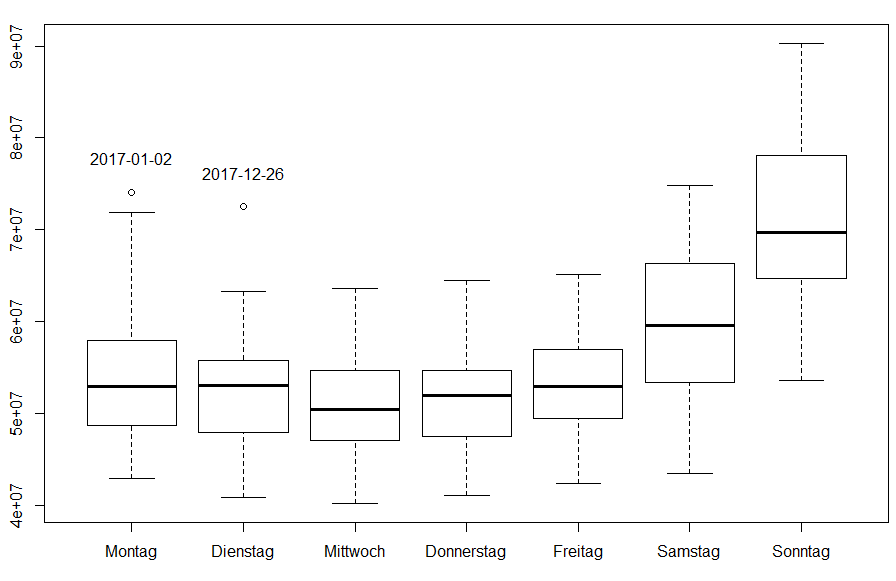
\includegraphics[width=0.75\linewidth]{../data/tv-week} 

}

\caption{\label{fig:fig1}The sum of TV viewing duration [seconds] by weekdays during 2017. On weekends more TV is watched than during the rest of the week. Festival days often behave like Sundays.}\label{fig:fig1}
\end{figure}

\begin{figure}[H]

{\centering 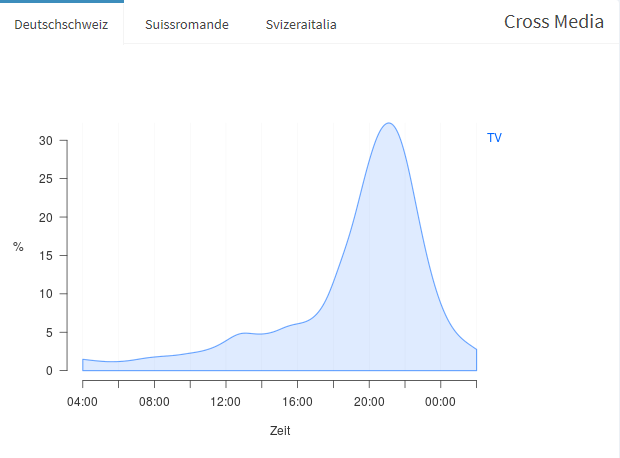
\includegraphics[width=0.75\linewidth]{../data/tv-day} 

}

\caption{\label{fig:fig2} The relative amount of TV viewing across time of the day. The curve is the average of all 365 days in 2017. In the market the peak around 20:00 o'clock is called Primetime. On weekends the curve is flatter.}\label{fig:fig2}
\end{figure}

\begin{figure}
\centering
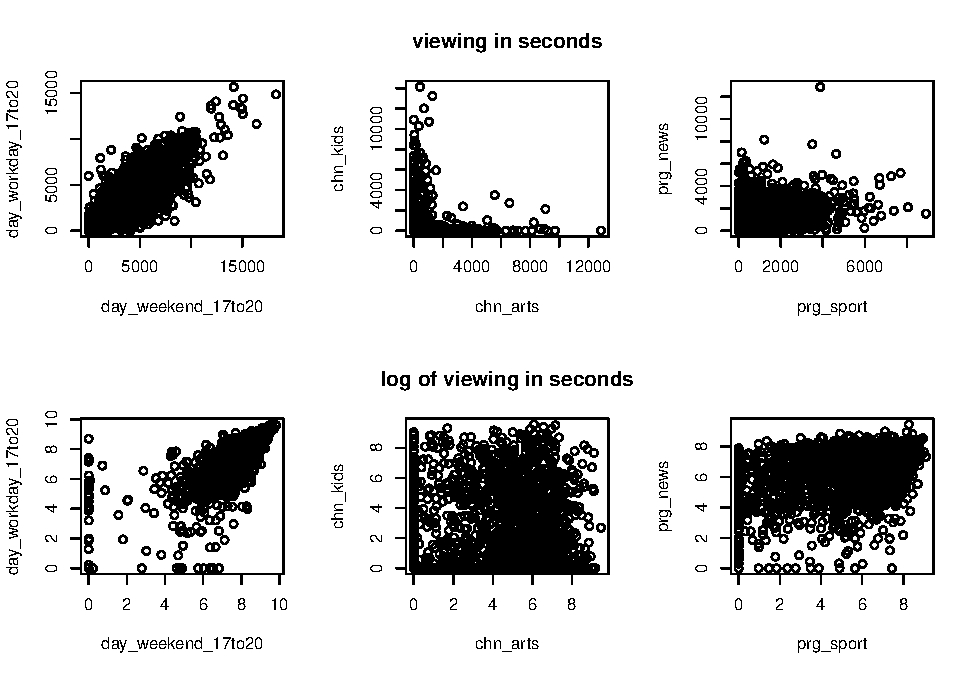
\includegraphics{Diploma_files/figure-latex/fig3-1.pdf}
\caption{\label{fig:fig3} Illustration of log transformation. The upper
row of scatterplots shows three examples of feature pairs. On of for
each domain \emph{time}, \emph{channel} and \emph{program}. In many
cases viewing duration is not symmetrical distributed. The lower row
shows the very same scatterplot with log transformed values.}
\end{figure}

\begin{figure}
\centering
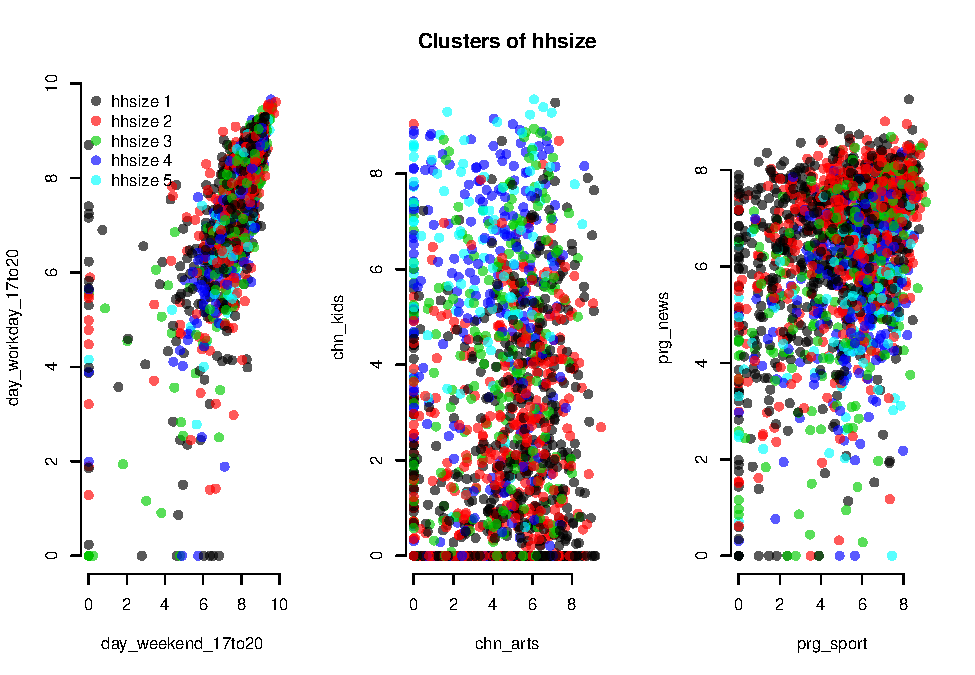
\includegraphics{Diploma_files/figure-latex/fig4-1.pdf}
\caption{\label{fig:fig4} Shown are the same three scatterplots as in
the Figure above but this time the corresponding household size is
indicated by the color of the dots. If there was a feature that would
separate the households (dots) into clusters of the same color, this
would tell us that this particular variable is a good discriminator for
household size. Apprently the variable \emph{chn\_kids} separates black
and red dots from light and dark blue dots. This means there is a
tendency that the more a household watches TV on typical kids channels,
the more likely it is a 4 or 5 person household.}
\end{figure}

\textbackslash{}begin\{figure\}{[}H{]}

\{\centering 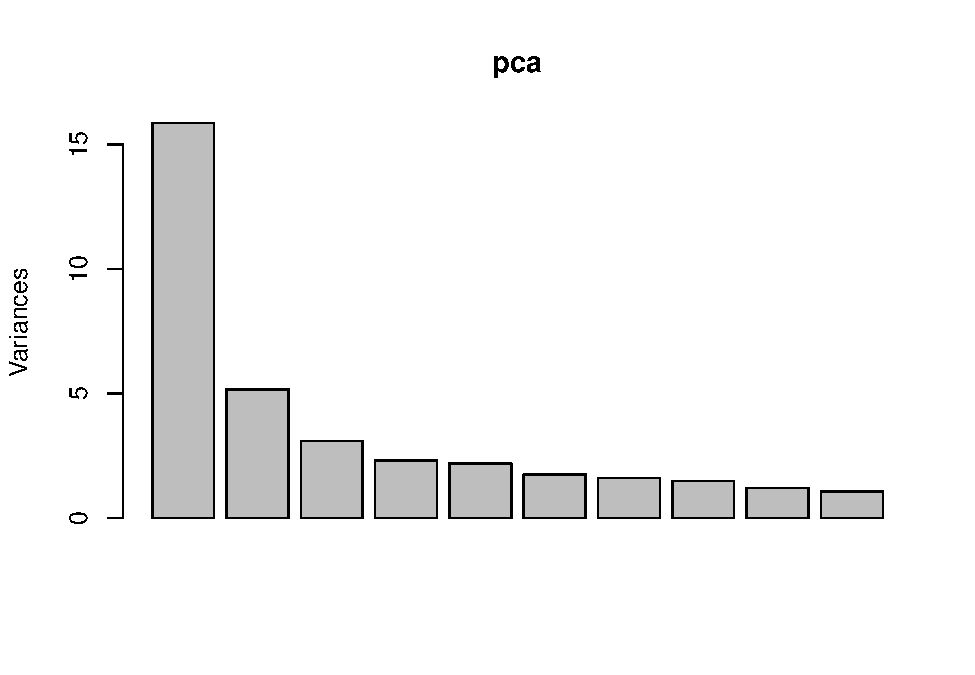
\includegraphics[width=0.5\linewidth]{Diploma_files/figure-latex/fig5-1}

\}

\textbackslash{}caption\{\label{fig:fig4} Principal Component Analysis
(PCA). Above the Screeplots shows the variance explained by the first 10
of principal components (PCs). The first PC explaine 30\% of the total
variance. Below, scatterplots and biplots of the first 3
PCs.\}\label{fig:fig5} \textbackslash{}end\{figure\}

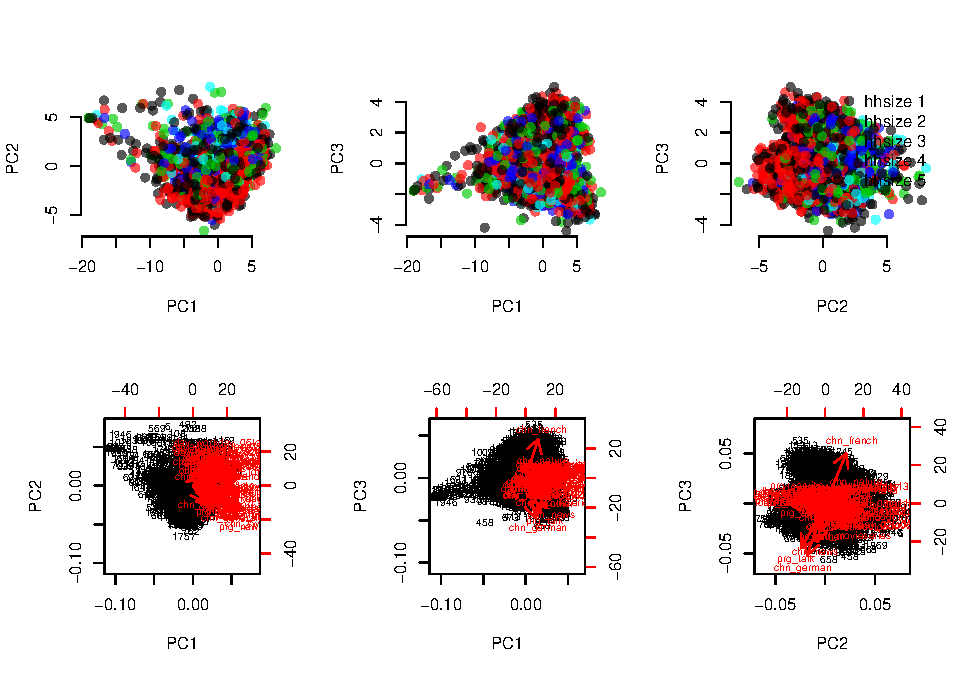
\includegraphics{Diploma_files/figure-latex/unnamed-chunk-6-1.pdf}


\end{document}
